\documentclass{article}

\usepackage{amsmath}
\usepackage{listings}
\usepackage{xcolor}
\usepackage{hyperref}

\usepackage{graphicx}
\usepackage{float}

\definecolor{commentcolor}{rgb}{0.0,0.5,0.0}
\definecolor{keywordcolor}{rgb}{0.0,0.0,0.6}
\definecolor{stringcolor}{rgb}{0.58,0.0,0.82}

\lstdefinelanguage{Haskell}{
  morekeywords={case,of,if,then,else,let,in,data,type,module,where,import,qualified,as,hiding,do,return},
  sensitive=true,
  morecomment=[l]--,
  morecomment=[s]{\{-}{-\}},
  morestring=[b]",
  morestring=[b]'
}

\lstset{
  language=Haskell,
  basicstyle=\ttfamily\small,
  keywordstyle=\color{keywordcolor}\bfseries,
  commentstyle=\color{commentcolor}\itshape,
  stringstyle=\color{stringcolor},
  numbers=left,
  numberstyle=\tiny\color{gray},
  stepnumber=1,
  numbersep=5pt,
  showstringspaces=false,
  tabsize=2,
  breaklines=true,
  frame=single,
  captionpos=b
}

\begin{document}

\title{Huffman Coding in Haskell}
\author{Rafał Włodarczyk, Michał Waluś}
\date{\today}

\maketitle

\tableofcontents
\newpage

\section{Introduction}
In 1952 David A. Huffman created an algorithm used for lossless data compression \cite{huffman1952method}, 
building upon the advances of Claude Shannon's work on information theory.
It has been proven to be optimal for symbol-by-symbol coding with a known
input probability distribution. The algorithm assigns variable-length codes to input characters, and the shorter codes are assigned to more frequently occurring characters.

\section{Initial Requirements}

The program has been designed to fulfill the following requirements:\\

Write a program that uses Huffman coding (classic or dynamic) to compress files.
This project will allow you to practice working with binary data and using tree-like data structures.
To handle binary data, you can use the \textit{bytestring} package.\\

\noindent
We decided that our take on the implementation will provide a simple command-line interface.

\subsection{Compression}

\paragraph{Compress:} Compresses the input file using Huffman encoding.
\begin{lstlisting}[language=bash]
$ huffman [input-file] -o [output-file]
\end{lstlisting}
Outputs the compression ratio and sizes.

\subsection{Decompression}

\paragraph{Decompress:} Decompresses the input file.
\begin{lstlisting}[language=bash]
$ huffman [input-file] -d -o [output-file]
\end{lstlisting}

\subsection{Parameters}
\begin{itemize}
    \item \textbf{[input-file]}: The file to be processed (required).
    \item \textbf{-o [output-file]}: Specifies the output file (required).
    \item \textbf{-d}: Enables decompression mode (default is compression).
\end{itemize}

\section{Huffman Coding Algorithm}

As described in \cite{wikihuffman}, can be summarized in the following steps:

\begin{enumerate}
    \item Count the frequency of each symbol in the input data.
    \item Create a leaf node for each symbol and add it to the priority queue.
    \item While there is more than one node in the queue:
        \begin{enumerate}
            \item Remove the two nodes of highest priority (lowest probability) from the queue.
            \item Create a new internal node with these two nodes as children and with probability equal to the sum of the two nodes' probabilities.
            \item Add the new node to the queue.
        \end{enumerate}
    \item The remaining node is the root node, and the tree is complete.
\end{enumerate}

\begin{figure}[H]
    \centering
    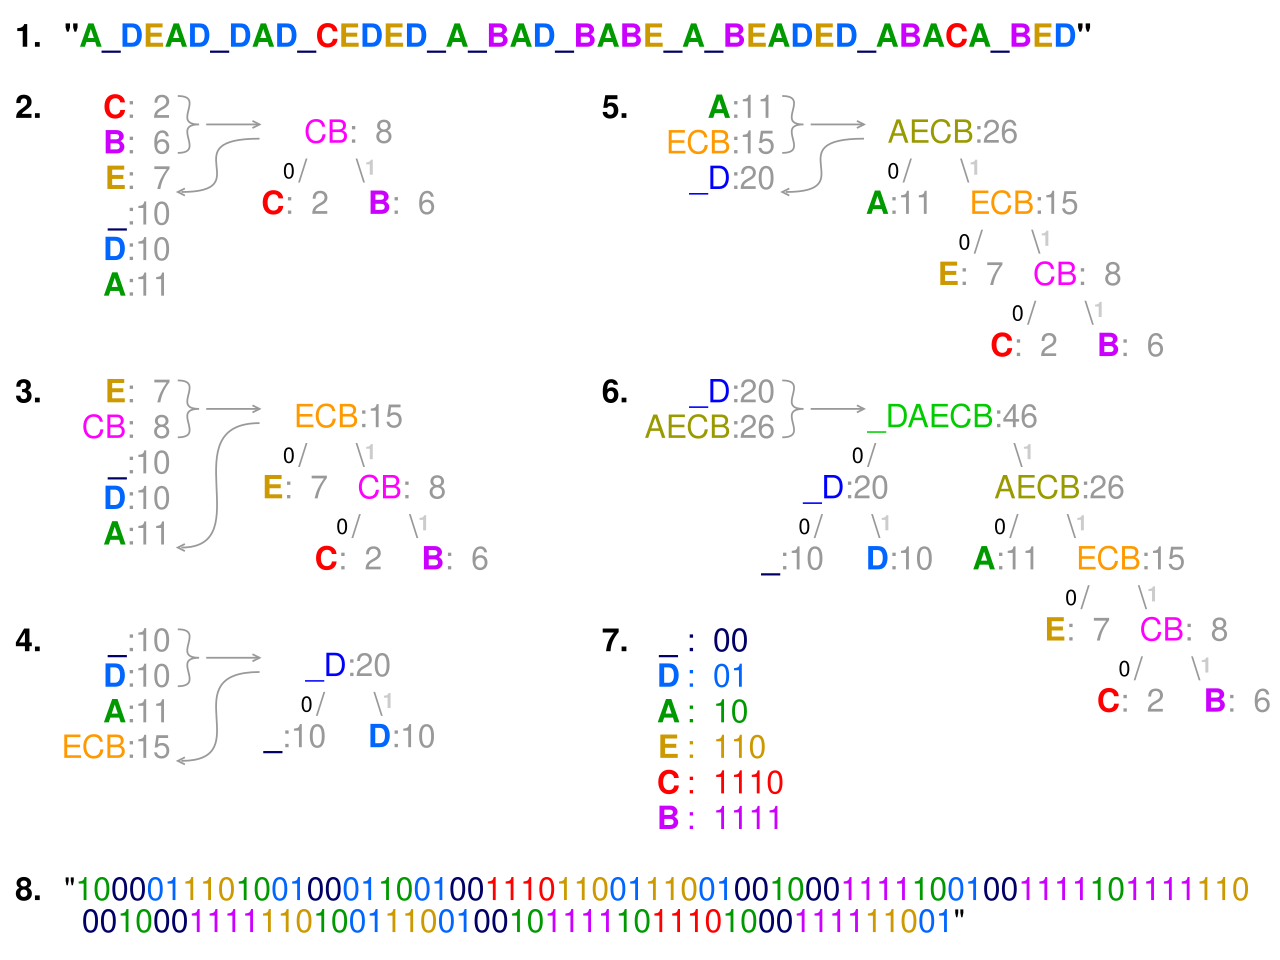
\includegraphics[width=0.8\textwidth]{schema.png}
    \caption{Huffman Coding Algorithm Schema}
    \label{fig:huffman-schema}
\end{figure}

\subsection{Prefix Codes}

A set of codes $\{C_1, C_2, \ldots, C_n\}$ is a prefix code if:
\begin{align}
    \forall i, j \in \{1, 2, \ldots, n\}, i \neq j: C_i \not\subseteq C_j
\end{align}

\noindent
In any stream of bits, defined as $S = b_1 b_2 \ldots b_m, b\in\{0,1\}$, 
a prefix code can be decoded unambiguously. This feature is crucial for
the Huffman coding algorithm as it allows deterministic decoding
of the compressed data in linear time.

\subsection{Frequency Map}

A frequency map assigns to each character in the input data the number of its occurrences.
For example, it can be easily constructed from a \textbf{String} intrinsic.

\begin{lstlisting}[language=Haskell, caption={Constructing a frequency map from a string.}]
type CharMap = [(Char, Int)]

add :: CharMap -> Char -> CharMap
add [] c = [(c, 1)]
add ((x, y):xs) c
    | x == c = (x, y + 1):xs
    | otherwise = (x, y):add xs c

mapChars :: String -> CharMap
mapChars = mapCharsHelp []
    where
        mapCharsHelp cm [] = cm
        mapCharsHelp cm (x:xs) = mapCharsHelp (add cm x) xs
\end{lstlisting}

\subsection{Priority Queue}

In order to build the Huffman tree in linear time, we must preserve the order of
the characters based on their number of occurrences. A priority queue is a data structure that allows for efficient insertion and extraction of the minimum element.

\begin{lstlisting}[language=Haskell, caption={Priority queue implementation using a binary tree.}]
type LeafQueue = [Tree Char Int]

createLQ :: String -> LeafQueue
createLQ = charMapToQueue . mapChars

insertLQ :: LeafQueue -> Tree Char Int -> LeafQueue
insertLQ [] tree = [tree]
insertLQ (t:lq) tree
    | get tree < get t = tree:t:lq
    | otherwise = t:insertLQ lq tree

mergeLQ :: LeafQueue -> Tree Char Int
mergeLQ [] = error "Cannot merge an empty queue"
mergeLQ [t] = t
mergeLQ (t1:t2:ts) = mergeLQ $ insertLQ ts $ Node t1 t2 $ get t1 + get t2

charMapToQueue :: CharMap -> LeafQueue
charMapToQueue = charMapToQueueHelp []
    where
        charMapToQueueHelp lq [] = lq
        charMapToQueueHelp lq ((c, i):cn) = charMapToQueueHelp (insertLQ lq $ Leaf c i) cn
\end{lstlisting}

\subsection{Huffman Tree construction}

We can now construct the Huffman tree (a binary tree with leaves containing characters) from the frequency map
each time extracting the two least frequent characters and merging them into a new node.

\begin{lstlisting}[language=Haskell, caption={Huffman tree construction.}]
data Tree a b = Leaf a b | Node (Tree a b) (Tree a b) b
    deriving (Eq)3_semester_2024
    makeCode :: Tree Char Int  -> Map Char String
    makeCode t = makeCodeHelp t ""
        where
            makeCodeHelp (Leaf x _) s = singleton x s
            makeCodeHelp (Node t1 t2 _) s = union (makeCodeHelp t1 (s ++ "0")) (makeCodeHelp t2 (s ++ "1"))
makeCode :: Tree Char Int  -> Map Char String
makeCode t = makeCodeHelp t ""
    where
        makeCodeHelp (Leaf x _) s = singleton x s
        makeCodeHelp (Node t1 t2 _) s = union (makeCodeHelp t1 (s ++ "0")) (makeCodeHelp t2 (s ++ "1"))
\end{lstlisting}

\subsection{Encoding and Decoding}

The encoding process is straightforward. we traverse the Huffman tree and replace each character with its corresponding code,
we decided to use a \textbf{Map} intrinsic to store the codes for each character. 
We can join the coding map with the input data to produce a compressed binary stream.

\subsection{Bytestream Operations}

The package \textbf{bytestring} provides an efficient way to handle binary data in Haskell.

\subsection{The Main Function}

The main function uses the IO monad to read the input file, perform processing and write the output file.

\section{CI}

\subsection{Build}

The project uses Stack as a build tool, which allows for simple dependency management and building.

\begin{lstlisting}[language=bash]
$ stack build
\end{lstlisting}

\subsection{Exec}

Afterwards, the executable can be run with the following command:

\begin{lstlisting}[language=bash]
$ stack exec huffman -- [input-file] -o [output-file]
\end{lstlisting}

\subsection{Bin}

To make it available globally, we can use \texttt{stack install}. 

\begin{lstlisting}[language=bash]
$ stack install
$ huffman
Usage: huffman <input-file> [-d] -o <output-file>
$ huffman src/Main.hs -o Main.hs.huff
src/Main.hs (1887 bytes) -> Main.hs.huff (1411 bytes) [74.77%]
\end{lstlisting}

\section{Showcase}

\begin{lstlisting}[language=bash]
$ wget https://pl.wikipedia.org/wiki/Polska -O polska.txt

$ sha256sum polska.txt
645e668ee...9c530  polska.txt

$ stack run -- polska.txt -o polska.txt.huff
polska.txt (1271161 bytes) -> polska.txt.huff (887871 bytes) [69.85%]

$ ls -lah polska.txt polska.txt.huff
-rw-r--r-- 1 rafisto rafisto 1.3M Jun  9 14:14 polska.txt
-rw-r--r-- 1 rafisto rafisto 868K Jun  9 23:27 polska.txt.huff

$ stack run -- polska.txt.huff -d -o polska.out.txt
polska.txt.huff (887871 bytes) -> polska.out.txt (1271161 bytes) [143.17%]

$ sha256sum polska.out.txt 
645e668ee...9c530  polska.out.txt
\end{lstlisting}

\section{Conclusions}

The Huffman coding algorithm with its presented implementation in Haskell has shown to be an effective way to compress text files.
We can assume a compression ratio of around 70\% for large text files, with the decompression process being lossless and efficient.

\section{Future Work}

The current implementation can be extended in several ways.
\begin{itemize}
    \item Optimization of the priority queue, library \textbf{containers} provides a more efficient implementation.
    \item As proposed by \cite{knuth1985dynamic}, dynamic Huffman coding allows data to be encoded without knowing the frequency distribution beforehand,
by maintaining a dynamic tree structure that adapts to the input data as it is processed.
\end{itemize}

\bibliographystyle{ieeetr}
\bibliography{docs}

\end{document}
